\section{Processi}\label{capitolo4}
In questo capitolo vedremo come i processi giochino un ruolo fondamentale nei sistemi distribuiti. Il concetto di processo proviene dall'ambito dei sistemi operativi ed è definito come un programma in esecuzione.\\
Per organizzare efficacemente un sistema client-server è spesso necessario utilizzare tecniche di \emph{multithreading} in quanto questa tecnica permette ai client e ai server di essere costruiti in modo tale che la comunicazione e l'elaborazione locale siano sovrapposti ottenendo un alto livello di prestazione.
\subsection{Thread}
Anche se i processi costituiscono la base di tutti i sistemi, la loro granularità non è sufficiente a soddisfare i bisogni dei sistemi distribuiti. una gestione più fine, sotto forma di \textbf{thread}, rende più facile la costruzione di applicazioni distribuite e ottenere prestazione migliori.
\subsubsection{Introduzione ai threads}
Prima di capire che cos'è un thread e che ruolo esso gioca nella costruzione di applicazioni distribuite è utile capire che cos'è in realtà un processo e che ruolo ha con i thread.\\
Per eseguire un programma, un sistema operativo crea un certo numero di processi virtuali. Per tener traccia di questi processi il sistema operativo mantiene aggiornata una \textbf{tabella dei processi} contenente elementi che vanno dalla memorizzazione dei registri della CPU, alla mappe della memoria, alla lista dei file aperti alle informazioni sugli \emph{account} e così via.\\
Il sistema operativo fa si che processi indipendenti non possano in alcun modo influire sulla correttezza degli altri processi, ovvero, è reso trasparente il fatto che più processi possano condividere concorrentemente la stessa CPU e le altre risorse hardware. Questa concorrenza però è ottenuta ad un prezzo abbastanza alto; ogni volta che viene creato un processo il sistema operativo deve creare uno spazio degli indirizzi completamente indipendente. Allocare memoria può voler dire inizializzare segmenti di memoria azzerando segmenti dati, copiare il programma in un segmento di testo e preparando uno \emph{stack} per i dati temporanei. Altrettanto costoso è il passaggio tra un processo ed un altro a livello di CPU, in quanto oltre a salvare il contesto è necessario cambiare i registri ed invalidare la cache.\\
Come un processo un \emph{thread} esegue il suo pezzo di codice indipendentemente dagli altri threads. A differenza dei processi nei threads non si cerca di ottenere un alto grado di trasparenza, in quanto il fatto di cercare di mantenere la trasparenza fa degradare le prestazione; di conseguenza un sistema basato sui thread gestisce l'insieme minimo delle informazioni per gestire la CPU. Infatti, il \textbf{contesto di un thread} è spesso costituito solamente dal contesto della CPU e dalle informazioni per gestire il thread stesso come ad esempio lo stato dovuto al blocco di una variabile \emph{mutex}. \uppercase{è} quindi compito degli sviluppatori proteggere l'accesso ai dati tra i vari threads di un singolo processo.
\paragraph{Utilizzo dei thread nei sistemi non distribuiti}
Il vantaggio principale dell'utilizzo dei thread nei sistemi non distribuiti deriva dal fatto che in un processo  a singolo thread quando viene effettuata una chiamata di sistema bloccante l'intero processo viene messo in pausa. Come nel caso di un foglio elettronico dove più celle sono collegate tra loro; in questo caso quando l'utente modifica il valore di una cella anche altre celle vengono rielaborate, ma tale rielaborazione è impensabile in un sistema a singolo thread in quanto il processo resterebbe bloccato in attesa di input e non calcolerebbe il valore delle altre celle.\\
Un altro vantaggio del multithreading è la possibilità di sfruttare il parallelismo quando si esegue il programma su sistemi multiprocessore. Il multithreading è usato anche nelle grandi applicazioni, le quali solitamente sono sviluppate come un insieme di processi cooperanti; tale cooperazione è realizzata tramite meccanismi di comunicazione tra processi (\emph{IPC, interprocess comunication}), ma questi meccanismi solitamente richiedono molti cambi di contesto che ne rallentano notevolmente le prestazioni. Invece di usare i processi un'applicazione può essere costruita mediante l'utilizzo di threads e la comunicazione tra questi avviene mediante l'uso dei dati condivisi, ed il passaggio da un thread all'altro può essere eseguito a livello utente.
\paragraph{Implementazione dei thread}
I thread sono spesso forniti sotto forma di pacchetto contente le operazioni di creazione e distruzione dei threads sia le operazioni per la loro sincronizzazione come \emph{mutex} e \emph{condition}. Gli approcci per implementare un pacchetto di thread sono due. Il primo è costruire una libreria che viene eseguita completamente a livello utente, il secondo è lasciare che il kernel sia conscio dei threads e si occupi del loro scheduling.\\
Usare una libreria utente ha notevoli vantaggi, prima di tutto la creazione e la distruzione dei threads a livello utente è molto meno costosa in quanto il costo è dovuto solo all'allocazione della memoria per creare uno \emph{stack}. Inoltre il cambio di contesto a livello utente può essere fatto con poche istruzioni. L'inconveniente principale dei thread a livello utente però è che una chiamata bloccante di sistema bloccherà l'intero processo e quindi bloccherà tutti i thread del processo.\\
Questo problema può essere raggirato implementando i threads a livello del kernel ma questo comporta che ogni operazione eseguita su un thread (creazione, distruzione, sincronizzazione e così via) dovrà essere eseguita a livello del kernel richiedendo quindi una chiamata a sistema che risulta essere molto più lenta e costosa come quella di un processo.\\
La soluzione ai problemi sta nell'uso di una forma ibrida chiamata \textbf{processi lightweight}. Un processo leggero viene eseguito nel contesto di un singolo processo (pesante) e per ogni processo ci possono essere più processi leggeri. Oltre a questi il sistema fornisce un pacchetto a livello utente per i threads mettendo a disposizione le solite operazioni. Il pacchetto dei thread è condivisibile da tutti i processi leggeri; questo significa che ogni processo leggero può eseguire il suo thread. Le applicazioni multithread vengono costruite creando dei thread e successivamente assegnando questi thread a un processo leggero.\\
Il pacchetto dei thread ha una singola routine per pianificare il thread successivo. Quando si crea un processo leggero gli si assegna uno \emph{stack} e lo si mette alla ricerca di un thread da eseguire. I thread in esecuzione sono sono salvati in una tabella in una tabella alla quale i processi leggeri accedono in mutua esclusione tramite l'uso di \emph{mutex} nello spazio utente. Questo significa che la sincronizzazione tra threads è interamente eseguita a livello utente senza la necessità di informare il kernel. \\
Nel caso in cui vi sia una chiamata di sistema bloccante il contesto di esecuzione passa dalla modalità utente a quella kernel ma continua comunque nel contesto del processo leggero attuale. Nel momento in cui il processo leggero non può più proseguire allora il sistema può decidere di proseguire con un altro processo leggero ritornando alla modalità utente.\\
I vantaggi di utilizzare un sistema ibrido sono molti. Innanzitutto la creazione, la distruzione e la sincronizzazione dei threads è relativamente poco costosa in quanto avviene a livello utente. Se un processo ha abbastanza processi leggeri allora una chiamata bloccante di sistema non bloccherà l'intero processo. A livello di architetture multiprocessore processi leggeri diversi possono essere eseguiti su CPU diverse.
L'unico inconveniente che si presenta è che i processi leggeri devono essere creati e distrutti ma fortunatamente tali operazioni non sono comuni.
\subsubsection{Thread nei sistemi distribuiti}
Come abbiamo visto il vantaggio principale dell'uso dei threads è che una chiamata di sistema bloccante non blocca l'intero processo. Questa caratteristica è molto vantaggiosa nel caso di realizzazione di comunicazioni multiple come ad esempio la gestione di comunicazioni client-server.
\paragraph{Client multithread}
Per raggiungere un buon grado di trasparenza alla distribuzione i sistemi distribuiti che operano su reti globali hanno la necessità di nascondere lunghi tempi di propagazione dei messaggi. La tecnica più comune per nascondere la latenza dei messaggi è quella di avviare la comunicazione ed immediatamente iniziare a fare qualcos'altro.
Un esempio molto diffuso sono i browser web che iniziano la comunicazione, ricevono una parte del codice HTML ed iniziano a visualizzare la pagina prima ancora di aver concluso la comunicazione.
\paragraph{Server multithread}
Anche se l'uso di client multithread offre notevoli vantaggi, il vero uso del multithreading è lato server. La pratica dimostra come l'uso del multithreading semplifica la codice e rende più facile lo sviluppo di applicazioni parallele per ottenere un alto livello di prestazioni.\\
Vediamo il caso di un \emph{file server} dove un \textbf{dispacher} riceve in ingresso su di una porta le richieste provenienti da diversi client. Dopo averla esaminata il dispacher seleziona un \textbf{worker thread} inattivo a cui assegnare la richiesta. Il \emph{worker} procede con la richiesta ed esegue una lettura bloccante sul file system locale; questo può far si che il thread vengo bloccato in attesa della lettura da disco, in tal caso viene selezionato un altro thread (\emph{worker} o \emph{dispacher}) che procede con la sua esecuzione.
\subsubsection{Il modello preemtive}
Nei sistemi moderni oltre ai thread viene utilizzato il modello \emph{preemtive}, ovvero è possibile forzare un processo ad abbandonare il suo stato di esecuzione. Solitamente questo meccanismo è utilizzato per implementare un meccanismo di \emph{time slicing} come mostrato in \figurename~\ref{fig:preemtive}.
\begin{figure}
\centering
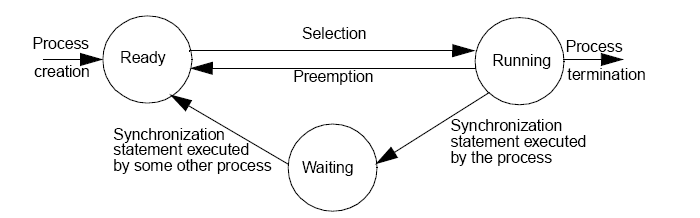
\includegraphics[scale=0.8]{img/preemtive.png}
\caption{Modello preemtive}\label{fig:preemtive}
\end{figure}
\subsection{I thread in C}
Tutti i sistemi UNIX sono multitasking con il sistema preemptive; tradizionalmente tutti i processi sono creati allo stesso modo tramite l'uso della primitiva \texttt{fork()}. La \emph{fork}produce una copia del processo chiamante; questa copia è esattamente identica all'origina tranne per il valore restituito dalla \texttt{fork} che per il processo figlio vale \emph{0} mentre nel padre il valore restituito è il \emph{pid} del figlio. Un piccolo esempio:
\begin{lstlisting}[language=C,float=htb,captionpos=b,caption={Esempio di uso della fork},label=lst:fork]
/*do parent stuff*/
ppid = fork ();
if (ppid < 0) {
	fork_error_function ();
} else if (ppid == 0) {
	child_function ();
} else {
	parent_function ();
}
\end{lstlisting}
La fork restituisce due copie completamente indipendenti dello stesso processo, questa indipendenza permette la protezione della memoria e la stabilità ma causa dei problemi quando si vuole che diversi processi lavorino sullo stesso problema; infatti sarebbe necessario usare \emph{pipes} oppure \emph{SysV IPC}. Inoltre il costo di switching tra processi multipli è molto alto, la sincronizzazione è lenta ed esistono dei limiti sul numero di processi che possono essere schedulati efficacemente.\\
Per questo sono stati introdotti i threads che invece possono essere schedulati all'interno del processo e risolvono molti problemi del lavoro multi processo.
L'API più popolare per creare una applicazione multithread in ambiente UNIX è la \emph{pthread} (\emph{POSIX thread}).\\
Le operazioni che si possono eseguire con quest'API sono la creazione, la distruzione, la sincronizzazione (\emph{join}), lo scheduling, il controllo dei dati e l'interazione con il processo principale. I threads dello stesso processo condividono le istruzioni di processo, gran parte dei dati, i descrittori dei file aperti, i segnali e lo user e il group id. Mentre per ogni thread abbiamo un distinto \emph{ThreadID}, un certo numero di registri, uno stack pointer ed una certa priorità come possiamo vedere \figurename~\ref{fig:threadstack}.
\begin{figure}[hbt]
\subfigure[]{
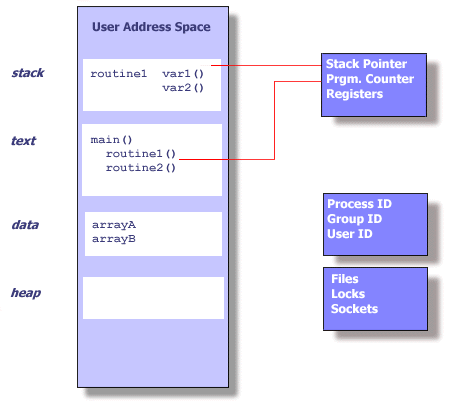
\includegraphics[width=7.5cm]{img/stack.png}
\label{fig:stack}
}
\subfigure[]{
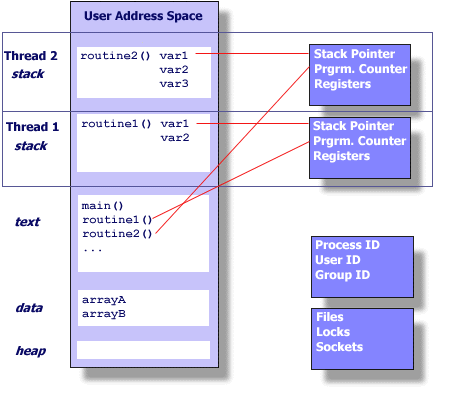
\includegraphics[width=7.5cm]{img/threadstack.png}
\label{fig:stackthread}
}
\caption{Memoria nel caso di processo (a) e di thread (b)}\label{fig:threadstack}
\end{figure}
Vediamo ora quali sono le funzioni della API \emph{pthread}
\paragraph{Thread creation}
La funzione per la creazione dei thread è:
\begin{lstlisting}[language=C,float=htb,captionpos=b,caption={Funzione di creazione dei thread},label=lst:creation]
int pthread_create (pthread_t *id, const pthread_attr_t *attr, void *(*routine)(void *), void *arg)
\end{lstlisting}
dove i valori sono:
\begin{description}
\item[id:] un valore che identifica il thread che viene restituito dalla funzione.
\item[attr]: un attributo che può essere utilizzato per impostare alcuni valori del thread. Se viene impostato a \emph{NULL} vengono impostati i valori di default.
\item[routine:] indica la funzione C che il thread eseguirà una volta creato.
\item[arg:] un singolo argomento che può essere passato a\texttt{routine}, deve essere passato come riferimento ad un puntatore di tipo \texttt{void}; in caso non vi siano valori si imposta a \emph{NULL}.
\end{description}
\paragraph{Thread termination}
Esistono diversi modi in cui un pthread può terminare:
\begin{itemize}
\item Il thread termina la sua routine.
\item Nel thread viene richiamata la \texttt{pthread\_exit}.
\item Il thread è cancellato da un altro thread tramite la chiamata della funzione \texttt{pthread\_cancel}.
\item L'intero processo termina quando viene chiamata una delle funzioni \texttt{exec} o \texttt{exit}.
\end{itemize}
Tramite la \texttt{pthread\_exit} è possibile specificare uno stato di terminazione che può essere restituito alla sincronizzazione del thread. Inoltre è molto importante ricordare che la \texttt{pthread\_exit} non chiude i file ed ogni file aperto all'interno del thread rimane aperto anche alla sua terminazione.
Se la funzione \emph{main} termina con una \texttt{pthread\_exit} prima che i threads siano conclusi i threads proseguono la loro esecuzione altrimenti terminano alla conclusione del \emph{main}.
Vediamo un esempio di creazione e terminazione dei thread in C nel Listato \ref{lst:thread}
\lstinputlisting[language=C,caption={Esempio di uso della API pthread},label=lst:thread]{listati/ThreadExample1.c}
\paragraph{Passaggio di argomenti}
Come abbiamo visto nella \emph{pthread\_create} è possibile impostare l'ultimo attributo con un attributo da passare alla routine che il thread eseguirà. Tale attributo deve essere convertito in un puntatore di tipo void. Tale passaggio presenta però alcuni tranelli, vediamo come nel Listato \ref{lst:wrongpass} come il passaggio per indirizzo crei un errore nell'esecuzione. Infatti, provando ad eseguire tale programma si rischia che più di un thread acceda contemporaneamente alla variabile \emph{t} e si rischiano quindi di ottenere dei valori sbagliati.
\begin{lstlisting}[language=C,caption={Errore nel passaggio di argomenti ad un thread},label=lst:wrongpass]
int rc, t;
for(t=0; t<NUM_THREADS; t++) {
	printf("Creating thread %d\n", t);
	rc = pthread_create(&threads[t], NULL, PrintHello, (void *) &t);
	...
}
\end{lstlisting}
Un possibile risultato di questo codice è quello seguente dove si può vedere che il thread numero 3 stampa il valore 4 anche se il thread numero 4 non è ancora stato creato (In realtà tutti i thread accedono alla variabile \emph{t} con un ritardo in quanto manca la stampa del thread numero 0).
\begin{verbatim}
Creazione del thread 0
Creazione del thread 1
1: Hello World!
Creazione del thread 2
2: Hello World!
Creazione del thread 3
3: Hello World!
4: Hello World!
Creazione del thread 4
\end{verbatim}
Per passare un argomento ad una routine è necessario controllare l'accesso ai dati da parte dei threads in modo che non vi siano possibili conflitti come nel caso del Listato \ref{lst:rightpass}. Nel quale viene passato ad ogni routine un puntatore ad un dato diverso.
\begin{lstlisting}[language=C,caption={Metodo corretto nel passaggio di argomenti ad un thread},label=lst:rightpass]
int *taskids[NUM_THREADS];
for(t=0; t<NUM_THREADS; t++) {
	taskids[t] = (int *) malloc(sizeof(int));
	*taskids[t] = t;
	printf("Creating thread %d\n", t);
	rc = pthread_create(&threads[t], NULL, PrintHello, (void *) taskids[t]);
	...
}
\end{lstlisting}
\paragraph{Joining threads}
L'operazione di \emph{join} è uno dei modi nel quale si può implementare la sincronizzazione tra thread.
\begin{lstlisting}[language=C]
int pthread_join(pthread_t thid,void **thread_return)
\end{lstlisting}
dove i diversi campi sono:
\begin{description}
\item[thid] è l'identificativo del thread su cui fare la join
\item[thread\_return] è il possibile valore di ritorno che si ottiene dall'invocazione della \texttt{pthread\_exit}
\end{description}
Il funzionamento della funzione di \emph{join} è specificato in \figurename\, \ref{fig:join}
\begin{figure}[htb]
\centering
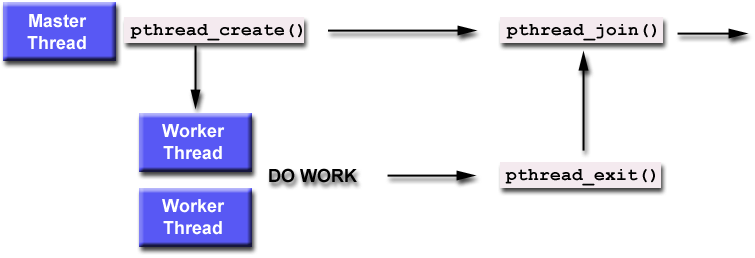
\includegraphics[scale=0.7]{img/join.png}
\caption{Funzionamento dell'operazione di join}\label{fig:join}
\end{figure}
\paragraph{I mutex}
Un \emph{mutex} funziona come un \emph{lock} proteggendo l'accesso a dei dati condivisi. Il concetto principale è che un solo thread alla volta può bloccare una variabile di tipo mutex, se più thread tenta di bloccare un mutex soltanto uno di questi effettuerà l'operazione con successo, inoltre i thread non possono bloccare un determinato mutex finché il thread che lo detiene non lo libera.\\
\uppercase{è} compito del programmatore assicurarsi che ogni thread che utilizza dei dati condivisi usi i mutex.\\
Una variabile di tipo mutex può essere dichiarata sfruttando la parola chiave \texttt{pthread\_mutex\_t}, per inizializzare tale variabile, invece, è possibile sfruttare due metodi:
\begin{itemize}
\item Il primo è l'inizializzazione statica come ad esempio
\begin{verbatim}
pthread_mutex_t mymutx = PTHREAD_MUTEX_INITIALIZER;
\end{verbatim}
\item Il secondo metodo è l'inizializzazione dinamica richiamando la routine
\begin{verbatim}
pthread_mutex_init
\end{verbatim}
In questo caso è possibile impostare alcuni parametri dell'oggetto mutex tramite le primitive \texttt{pthread\_mutexattr\_init} e \texttt{pthread\_mutexattr\_destroy} che rispettivamente creano e distruggono gli attributi  di un mutex
\end{itemize}
In entrambi i casi di inizializzazione l'oggetto mutex è inizializzato \emph{unlocked}. Infine, la routine \texttt{pthread\_mutex\_destroy} permette di rilasciare un mutex di cui non si ha più bisogno.\\
Esistono tre primitive per la gestione dei mutex, queste sono:
\begin{itemize}
\item \texttt{pthread\_mutex\_lock:} che si usa per acquisire un lock su di una variabile, nel caso in cui tale lock sia detenuto da un altro thread il thread che ha richiesto il lock si blocca finché il blocco non viene rilasciato.
\item \texttt{pthread\_mutex\_trylock} molto simile alla routine precedente solo che nel caso in cui il blocco sia detenuto da un altro thread allora la routine restituisce un codice di errore che indica \emph{"busy"}; è molto utile nel caso si vogliano prevenire condizioni di deadlock.
\item \texttt{pthread\_mutex\_unlock:} questa routine permette di rilasciare il lock in possesso del thread ma restituisce un errore nel caso in cui si voglia rilasciare un lock su di una variabile già sbloccata o bloccata da un altro thread.
\end{itemize}
\lstinputlisting[language=C,caption={Esempio di uso delle variabili mutex},label=lst:mutex]{listati/ThreadExample2.c}
\paragraph{Condition variables}
Mentre i mutex implementano la sincronizzazione tramite il controllo degli accessi sui dati le \emph{condition variables} permettono ai thread di sincronizzarsi in base ad un determinato valore di un dato. Senza quest'aspetto dei thread bisognerebbe implementare un polling per verificare quando una particolare condizione viene riscontrata. Le \emph{condition variables} sono un modo per ottenere lo stesso risultato senza il polling, e possono essere utilizzate anche insieme ai mutex.
L'utilizzo principale sono tutti quei problemi della categoria\textbf{produttore-consumatore}.\\
Come per i mutex le condition variabile sono dichiarate utilizzando la parola chiave \texttt{pthread\_cond\_t}; per l'inizializzazione esistono due metodi:
\begin{itemize}
\item Statico
\begin{verbatim}
pthread_cond_t myconvar = PTHREAD_COND_INITIALIZER
\end{verbatim}
\item Dinamico tramite la funzione \texttt{pthread\_cond\_init} che permette di settare anche gli attributi della variabile tramite le due primitive
\begin{verbatim}
pthread_condattr_init
pthread_condattr_destroy
\end{verbatim}
Che permettono rispettivamente di inizializzare e distruggere gli attributi della variabile
\end{itemize}
Infine tramite la primitiva \texttt{pthread\_cond\_destroy} è possibile liberare una variabile condizionale che non è più necessaria.\\
Per la gestione di questo tipo di variabile esistono diverse primitive:
\begin{itemize}
\item \texttt{pthread\_cond\_wait} è una routine che il thread finché una determinata condizione non si verifica, se chiamata quando vi è un lock attivo la routine sblocca il mutex e lo blocca nuovamente quando il thread si sveglia.
\item \texttt{pthread\_cond\_signal} questa routine risveglia gli altri thread in attesa di una \emph{condition variables}
\item \texttt{pthread\_cond\_brodcast} può essere utilizzata al posto della routine precedente se ci sono più thread bloccati in uno stato di \emph{"wait"}.
\end{itemize}
\subsection{Concorrenza in Java}
Come per il C anche il Java fornisce il supporto alla concorrenza a livello di linguaggio, esso mette a disposizione delle classi per istanziare ed eseguire nuovi thread più i metodi di sincronizzazione e le variabili di condizione.
Il modo più semplice per creare un thread è quello di utilizzare la classe \texttt{java.lang.Thread} in questo caso è sempre necessario implementare un metodo \texttt{run()}.
\begin{lstlisting}[language=Java,caption={Uso della classe Thread in Java},label=lst:jthread]
public class MyThread extends Thread {
	private String message;
	public MyThread(String m) {message = m;}
	public void run() {
		for(int r=0; r<20; r++)
			System.out.println(message);
	}
}

public class ProvaThread {
	public static void main(String[] args) {
		MyThread t1,t2;
		t1=new MyThread("primo thread");
		t2=new MyThread("secondo thread");
		t1.start();
		t2.start();
	}
}
\end{lstlisting}
Come vediamo la nostra classe che implementa un thread estende l'oggetto \emph{Thread}, in questa classe viene fatto l'override del metodo \texttt{run()} il quale non è altro che la routine che viene eseguita dal thread. Per far partire il thread è necessario richiamare il metodo \texttt{start()} dopo aver creato un nuovo oggetto.\\
Un'altra possibile soluzione è l'utilizzo dell'interfaccia \texttt{Runnable} la quale specifica soltanto che deve esistere un metodo \texttt{run()} che deve essere implementato. La classe \texttt{Thread} implementa anch'essa l'interfaccia \texttt{Runnable}.
Come vediamo nel Listato\,\ref{lst:runnable} a differenza del caso precedente oltre all'oggetto \emph{MyThread} deve anche essere creato un oggetto \emph{Thread} corrispondente, al quale viene poi passato l'oggetto MyThread, ed infine il metodo \texttt{start()}viene invocato sull'oggetto Thread.
\lstinputlisting[language=Java,caption={Utilizzo dell'interfaccia Runnable},label=lst:runnable]{listati/MyThread.java}
L'esecuzione dei thread non segue un ordine predefinito ma lo stesso codice può produrre risultati diversi su diversi computer o addirittura sullo stesso. Questo caratteristica è chiamata \emph{non-determinismo} ed è un punto focale nella concorrenza.\\
Java di per se implementa il modello \emph{preemtive} e nel caso sia disponibile un meccanismo di \emph{time-slicing} allora java esegue i thread con la stessa priorità tramite una meccanismo di \emph{round-robin}.\\
Per definire quando un sistema multithread è corretto si devono rispettare due proprietà:
\begin{itemize}
\item\emph{Sicurezza:} Un sistema si dice sicuro quando gli eventi malevoli non accadono.
\item\emph{Longevità:} Un sistema è longevo quando le cose buone possono accadere.
\end{itemize}
I possibili guasti che rientrano nella categoria "Sicurezza" sono quei guasti che avvengono a livello di esecuzione come i conflitti \emph{read/write} e \emph{write/write}. I meccanismi che invece riguardano la "Longevità" sono quei meccanismi che bloccano l'esecuzione del programma come:
\begin{itemize}
\item Lock
\item Waiting
\item CPU contention
\end{itemize}
Solitamente, purtroppo, le cose più semplici che si possono fare per aumentare la longevità ne riducono però la sicurezza e vice versa.\\
Vediamo ora quali sono i meccanismi che Java mette a disposizione per supportare la concorrenza.
\paragraph{Exclusion}
In un sistema sicuro ogni oggetto protegge se stesso da possibili violazioni della sua integrità. le tecniche di esclusione preservano l'invariante di un oggetto. Tre sono le tecniche principali per permettere l'\emph{esclusione}:
\begin{itemize}
\item Immutabilità
\item Esclusione dinamica (Locking)
\item Esclusione strutturale
\end{itemize}
Per quanto riguarda l'\textbf{immutabilità} si ottiene creando le classi in modo che gli oggetti proteggano se stessi come nel Listato\,\ref{lst:immutabile}
\begin{lstlisting}[language=Java,caption={Esempio di oggetto immutabile},label=lst:immutabile]
class ImmutableAdder {
	private final int offset;
	public Immutableadder (int a) {
		offset = a;
	}
	public int addOffset (int b) {
		return offset + b;
	}
}
\end{lstlisting}
I vantaggi di questa tecnica sono il fatto che non richiede sincronizzazione ed è molto utile per condividere degli oggetti tra i threads, ma sfortunatamente ha dei limiti di applicabilità.\\
Per parlare di sincronizzazione introduciamo prima l'esempio del Listato\,\ref{lst:sincro}
\begin{lstlisting}[language=Java,caption={Esempio sincronizzazione},label=lst:sincro]
public class RGBColor {
	private int r;
	private int g;
	private int b;
	
	public void setColor (int r, int g, int b)
		checkRGBVals(r, g, b);
		this.r = r;
		this.g = g;
		this.b = b;
	}
}
\end{lstlisting}
Ora immaginiamo che due thread chiamati \emph{red} e \emph{blue} vogliano impostare contemporaneamente il loro colore sullo stesso oggetto di tipo \texttt{RGBColor} a questo punto potrebbero verificarsi dei problemi in quanto i due thread tentano di scrivere lo stesso dato violando così la sua integrità.\\
Per risolvere questo problema java tramite il locking serializza l'esecuzione del codice dichiarato \emph{synchronized}. Ogni istanza di un oggetto possiede tali meccanismi di lock in quanto derivati dalla classe \texttt{Object}, l'unica eccezione si ha con l'utilizzo di array, infatti, bloccare un array non blocca gli elementi di tale array.\\
Esistono due modi per bloccare una parte di codice, si può dichiarare \emph{synchronized} un intero metodo o un singolo blocco di codice, in caso di singolo blocco la funzione \texttt{synchronized} richiede l'oggetto sul quale effettuare il lock (Listato\,\ref{lst:syncobj} e Listato\,\ref{lst:syncmeto}).\\
\pagebreak
\begin{lstlisting}[language=Java,caption={Sincronizzazione di una parte di codice},label=lst:syncobj]
synchronized (object) {
	//Lock is held
	...
}
//Lock is released
\end{lstlisting}
\begin{lstlisting}[language=Java,caption={Sincronizzazione di un metodo},label=lst:syncmeto]
synchronized void f() {
	//Lock is held
	/* Body */
}
//Lock is released
\end{lstlisting}
I lock vengono automaticamente acquisiti all'ingresso del blocco o del metodo dichiarato \texttt{synchronized} e rilasciato all'uscita da esso.\\
Alcune regole chiave per l'uso della sincronizzazione sono:
\begin{itemize}
\item Sempre quando si effettua un aggiornamento a dei campi di un oggetto.
\begin{lstlisting}[language=Java]
synchronized (point) {
	point.x = 5; point.y = 7;
}
\end{lstlisting}
\item Tutte le volte che si accede a dei dati che potrebbero essere aggiornati.
\begin{lstlisting}[language=Java]
synchronized (point) {
	if (point.x > 0) {...}
}
\end{lstlisting}
\item Si può fare a meno di sincronizzare parti di metodo stateless
\begin{lstlisting}[language=Java]
public void f() {
	synchronized (this) {
		state = ...;
	}
	operations();
}
\end{lstlisting}
\item \textbf{Mai} sincronizzare parti di codice che contengono invocazioni ad altri oggetti
\begin{lstlisting}[language=Java]
public void f() {
	synchronized (this) {
		...
	}
	h.foo();
}
\end{lstlisting}
\end{itemize}
La strategia più sicura (ma non la più efficace) per realizzare un'applicazione OO concorrente è quella di utilizzare oggetti completamente sincronizzati, anche detti oggetti \emph{atomici}, nei quali tutti i metodi sono sincronizzati, non esistono campi pubblici o altri tipi di violazione nell'incapsulamento, tutti i metodi sono finiti e hanno modo di rilasciare il lock, tutti i campi sono inizializzati ad un valore consistente nel costruttore, ed infine lo stato dell'oggetto è consistente sia all'inizio che alla fine di ogni metodo anche in presenza di eccezioni.\\
Uno dei problemi principali della programmazione concorrente è il \emph{deadlock}, tale problema si verifica quando due o più oggetti sono acceduti da due o più threads e tali thread detengono un lock mentre tentano di acquisire un lock detenuto da un altro thread.\\
L'assegnamento di un valore ad una variabile è un'operazione atomica (a parte per i \emph{long} e i \emph{double}), questo significa che generalmente non è necessario sincronizzare l'accesso ad una variabile. Tuttavia i thread solitamente memorizzano il valori delle variabile in memoria locale, questo significa che se un thread cambia il valore di una variabile un altro thread non vede il cambiamento. Per evitare questo meccanismo bisogna sincronizzare la variabile oppure dichiararla di tipo \texttt{volatile} che significa che ogni volta che una variabile è usata deve prima essere letta dalla memoria principale.\\
Il confinamento implementa l'incapsulamento garantendo che al massimo un'attività alla volta acceda agli oggetti. Questo meccanismo permette l'accesso ad un solo thread alla volta senza utilizzare i locking dinamici.
Il punto principale è quello avere un punto di uscita dal thread. Esistono quattro categorie per verificare che un riferimento \emph{r} ad un oggetto \emph{x} può uscire da un metodo \emph{m}:
\begin{itemize}
\item \emph{m} passa \emph{r} come argomento di un'invocazione ad un metodo o ad un costruttore di un oggetto
\item \emph{m} passa \emph{r} come valore di ritorno di un metodo.
\item \emph{m} registra \emph{r} in un campo accessibile da altre attività
\item \emph{m} rilascia un riferimento che però permette l'accesso ad \emph{r}
\end{itemize}
Per quanto riguarda le collezioni, il framework \texttt{java.util.Collection}  basata su uno schema \emph{Adapter} permette la sincronizzazioni delle classi collection, infatti, ad eccezione di \texttt{Vector} e \texttt{Hashtable} le classi base per le collezioni (come \texttt{java.utili.ArrayList}) sono non sincronizzate. Sono state così costruite una serie di classi sincronizzate attorno alle classi base come la \texttt{Collection.synchronizedList}.\\
Come abbiamo detto prima però la sincronizzazione non è molto efficiente infatti richiamare un metodo sincronizzato richiede un tempo quattro volte maggiore rispetto a metodi non sincronizzati; inoltre, esso riduce la concorrenza e diminuisce le performance, infine non vi è alcun modo di controllare il meccanismo dei lock.\\
Con java versione 5 sono stati introdotti nuovi meccanismi di sincronizzazione come la \emph{sincronizzazione condizionata.} Prendiamo come esempio un parcheggio con una certa capacità e dei metodi che permettono l'arrivo e la partenza di automobili come esemplificato nel Listato\,\ref{lst:monitor}.
\begin{lstlisting} [language=Java,caption={Esempio di controllore di un parcheggio},label=lst:monitor]
public class CarParkControl {
	protected int space;
	protected int capacity;
	
	public CarParckControl (int n) {
		capacity = space = n;
	}
	
	syncronized public void arrive() {
		...; --space; ...;
	}
	syncronized public void depart() {
		...; ++space; ...;
	}
}
\end{lstlisting}
Come per il C esistono però dei metodi che permettono una gestione più efficiente del controllore rispetto all'uso della syncronized; questi metodi sono:
\begin{itemize}
\item \texttt{public final void notify()}: che risveglia un singolo thread in attesa.
\item \texttt{public final void notifyAll()}: risveglia tutti i thread in attesa.
\item \texttt{public final void wait() throws InterruptedException}: pone il thread in attesa di un \emph{notify}. Quando un thread viene posto in uno stato di wait esso rilascia il lock acquisito e lo riacquista al suo risveglio.
\end{itemize}
\lstinputlisting[language=Java,caption={Esempio di variabili condizionali in Java},label=lst:jsincro]{listati/CarParkControl.java}
Si può ridurre l'overhead dovuto al contex-switching sostituendo la \texttt{notifyAll} con la \texttt{notify}. Tale meccanismo può essere usato per migliorare le performance quando si è certi che almeno un thread è in atteso per eseguire un lavoro.\\
Alla condizione di \emph{wait} è possibile associare un timer molto utile per migliorare la longevità del sistema in quanto tende a risolvere in modo automatico i deadlock.